\fuxiti
\begin{xiaotis}

\xiaoti{“水是由氢气和氧气组成的”。
    “水分子是由一个氢分子和一个氧原子组成的”。
    “水是由氢氧两种分子组成的"。
    这些说法对不对?为什么?正确的应该怎样说?用什么方法把水变成氢气和氧气?
}

\xiaoti{下列各混和气体点燃时,哪个可能爆炸,哪个不能?为什么?
    (假定能爆炸的混和气体组成比均在爆炸极限之内。)
}
\begin{xiaoxiaotis}

    \xxt{氢气和氧气的混和气体,}

    \xxt{氢气和氦气的混和气体,}

    \xxt{氧气和氮气的混和气体,}

    \xxt{氢气和空气的混和气体。}

\end{xiaoxiaotis}


\xiaoti{有人设计了实验室制取氢气的简易装置(见下图), 哪种是正确的.哪种是错误的?为什么?}

\begin{figure}[htbp]
    \centering
    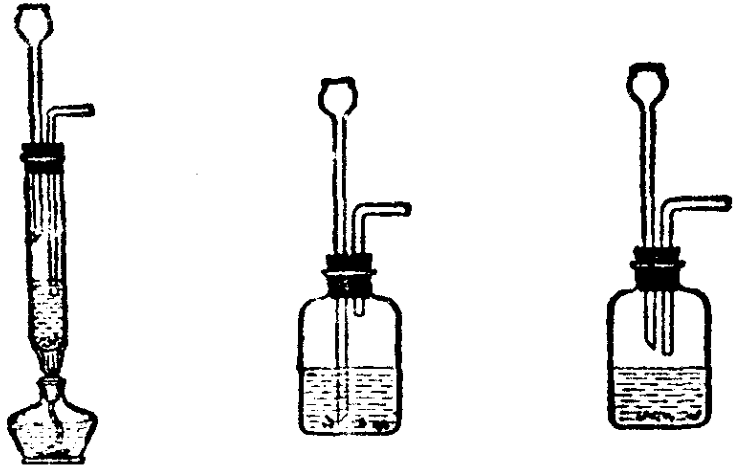
\includegraphics[width=9cm]{../pic/czhx1-ch2-fuxi-3}
\end{figure}


\xiaoti{写出下列结构示意图所代表的原子或离子的符号:}
\begin{xiaoxiaotis}
    \newcommand{\yuanzi}[2]{
        \stepcounter{cntxiaoxiaoti}
        \tikz [scale=0.9]{
            \pic  [local bounding box=A1, transform shape] at (0, 0) {atom={#1}};
            \draw ($(A1.east) + (0.1, 0)$) -- +(1, 0) node[right] {#2};
            \draw ($(A1.west) + (-0.2, 0)$) node[left] {\labelxiaoxiaoti};
        }
    }

    \begin{tblr}{colsep=0pt}
        \yuanzi{number=8,layer={2,8}}{,}    & \yuanzi{number=9,layer={2,8}}{,}  & \yuanzi{number=10}{,} \\
    \end{tblr}

    \begin{tblr}{colsep=0pt}
        \yuanzi{number=11,layer={2,8}}{,}   & \yuanzi{number=15}{,}             & \yuanzi{number=16,layer={2,8,8}}{,} \\
        \yuanzi{number=17,layer={2,8,8}}{,} & \yuanzi{number=18}{。}
    \end{tblr}

\end{xiaoxiaotis}


\xiaoti{选择正确的答案填写在括号里:}
\begin{xiaoxiaotis}

    \xxt{元素的化学性质主要决定于原子的 \ewkh 。\\
        \tc{1} 核外电子层数, \tc{2} 最外层电子数, \tc{3} 核内中子数。
    }

    \xxt{硫化钠(\ce{Na2S}) 是 \ewkh 。\\
        \tc{1} 共价化合物, \tc{2} 混和物, \tc{3} 离子化合物。
    }

    \xxt{在 \ce{H2SO4} 中硫的化合价是 \ewkh 。\\
        \tc{1} $-2$ 价, \tc{2} $+4$ 价, \tc{3} $+6$ 价。
    }

    \xxt{氮在 \ce{NO2} 中的化合价是 \ewkh, 在 \ce{NH3} 中的化合价是 \ewkh。\\
        \tc{1} $-3$ 价, \tc{2} $+2$ 价, \tc{3} $+4$ 价, \tc{4} $+5$ 价。
    }

\end{xiaoxiaotis}


\xiaoti{某化工厂需要 5 吨氧气作原料,这些氧气用电解水的方法制得。
    这需要消耗多少吨水?同时还可以产生多少吨氢气?
    这些氢气跟足量氯气反应,又可以合成多少吨氯化氢?
}

\xiaoti{把干燥纯净的氯酸钾和二氧化锰的混和物 15.5 克装入大试管,给试管加热来制取氧气。
    在反应不再发生后,等试管冷却,称量,得 10.7 克固体物质。问:
    (1)制得氧气多少克?
    (2) 10.7 克固体物质里含有哪些物质?各多少克?
}

\end{xiaotis}

